%TODO: in general, this chapter could need a few more references to concepts / statements; I marked a few bit down the text, but there are other occasions where it fits

\chapter{Background}
\label{ch:background}

This chapter aims to equip the reader with the necessary background for the rest of the work. The definitions are formulated in a mathematical way. We expect the reader to be familiar with the notation.

\section{Machine Learning}
\label{sec:machinelearning}

\textit{Machine Learning} (ML) is a subfield of Artificial Intelligence (AI) and was defined by Tom Mitchell as "the study of computer algorithms that allow computer programs to automatically improve through experience" \cite{mitchell_machine_1997}.

The main objective in ML is the problem $\mathcal{P}$, i.e. the task that the ML model is trained to solve. %Such a problem $\mathcal{P}$ could be, e.g., classifying handwritten digits (image classification), grouping people based on different properties in order to identify outliers (clustering, anomaly detection) or solving a maze.
Common problems in ML are \cite{mohri_foundations_2018}:
% mehr oder weniger kopiert aus \cite{mohri_foundations_2018}
\begin{itemize}
    \item \textit{Classification}: "this is the problem of assigning a category to each example. For example, document classification consists of assigning a category such as politics, business, sports, or weather to each document, while image classification consists of assigning to each image a category such as car, train, or plane. The number of categories in such tasks is often less than a few hundred, but it can be much larger in some difficult tasks such as in text classification or speech recognition."
    % todo some math behind classification?
    \item \textit{Regression}: "this is the problem of predicting a real value for each item. Examples of regression include prediction of stock values or that of variations of economic variables. In regression, the penalty for an incorrect prediction depends on the magnitude of the difference between the true and predicted values, in contrast with the classification problem, where there is typically no notion of similarity between various categories."
    \item \textit{Clustering}: "this is the problem of partitioning a set of items into homogeneous subsets. Clustering is often used to analyse very large data sets. For example, in the context of social network analysis, clustering algorithms attempt to identify natural communities within large groups of people."
    %\item \textit{Dimensionality reduction}: this problem consists of transforming an initial representation of items into a lower-dimensional representation while preserving some properties of the initial representation. A common example is the Principal Component Analysis (PCA).
\end{itemize}

These problems are usually assigned to one of the three main categories in ML (cf. \cref{fig:machine_learning_structure}):

\begin{enumerate}
    \item \textbf{Supervised Learning} -- the model learns to make predictions based on a set of labelled data, e.g. classification or regression.
    \item \textbf{Unsupervised Learning} -- the model learns to find patterns in an unlabelled dataset, e.g. clustering or dimensionality reduction.
    \item \textbf{Reinforcement Learning} -- the model learns to master a task based on a feedback loop, e.g. playing a game.
\end{enumerate}

\begin{figure} %[H]
    \centering
    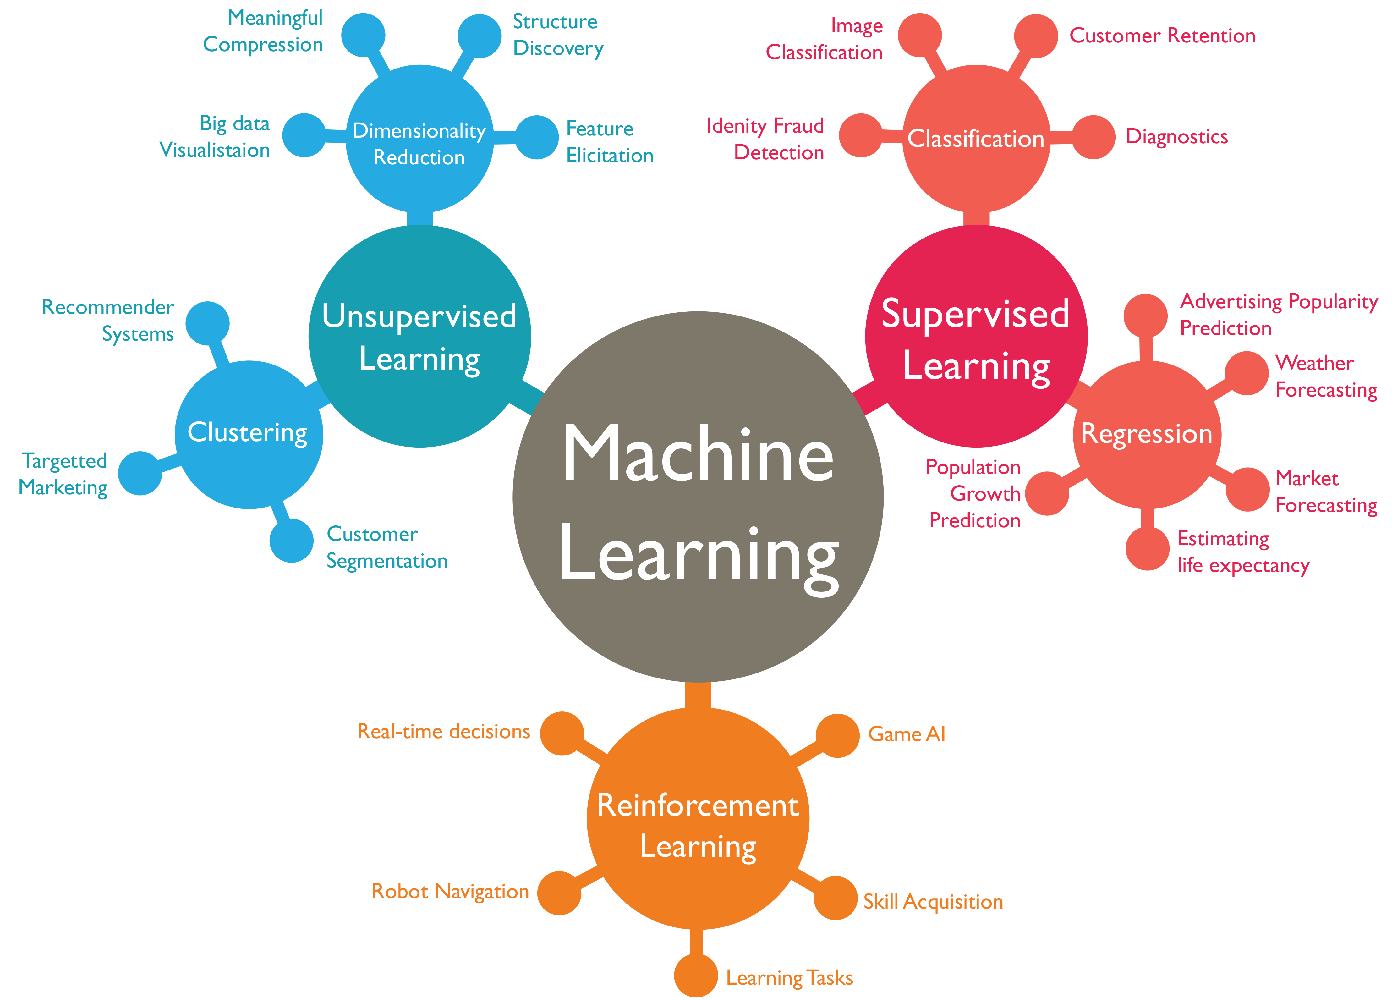
\includegraphics[width=.75\linewidth]{images/machine-learning.png}
    \caption{Three main categories of ML, their algorithms and use cases. Source: \cite{shewan_10_nodate}}
    \label{fig:machine_learning_structure}
\end{figure}

%Current research on Model Watermarking and therefore the thesis focuses on image classification. Image classification or image recognition is the most common application for Supervised Learning. Before we will dive into image classification and neural networks, w
We define typical terminology for Machine Learning \cite{mohri_foundations_2018}:
% mehr oder weniger kopiert aus \cite{mohri_foundations_2018}
\begin{itemize}
    \item \textit{Examples}: "Items or instances of data used for learning or testing. In image classification, these examples are images which we will use for learning and testing."
    \item \textit{Labels}: "Values or categories assigned to examples. In image classification, examples are assigned specific categories, for instance, car, train or plane."
    \item \textit{Parameters:} are values that control the behaviour of an ML model and are the instances that are updated during model training. We denote parameters, often also called \textit{weights}, by a vector $\mathbf{w}$, but also $\theta$ is a commonly used notation. 
    \item \textit{Hyperparameters}: "Free parameters that are not determined by the learning algorithm, but rather specified as inputs to the learning algorithm, such as the learning rate or the batch size."
    \item \textit{Training set}: "Examples or example-label pairs used to train a learning algorithm."
    \item \textit{Validation set}: "Examples or example-label pairs used to select appropriate values for the learning algorithm’s hyperparameters", or early stopping. Early stopping is a mechanism to stop training when the validation set performs best, in order to prevent from overfitting (cf. \cref{sec:overfitting}).
    \item \textit{Test set}: "Examples or example-label pairs used to evaluate the effectiveness of a learning algorithm. The test set is separate from the training and validation set and is not made available in the learning stage." The training, validation and test sets are pairwise disjoint subsets of the dataset. In Supervised Learning, the training, validation and test sets consist of example-label pairs, in unsupervised learning, on the other hand, only of examples.
    \item \textit{Loss function}: "A function, that measures the difference, or \textit{loss}, between a predicted label and a true label." We denote the loss function as $\mathcal{L}(\mathbf{w})$, where $\mathbf{w}$ is the ML model's parameter vector, since we usually want to minimise the loss function according to the model's parameters $\mathbf{w}$ (cf. \cref{eq:regression_loss}). However, in practice, the loss function is computed with the input of the true label and predicted label, and could therefore be denoted as $\mathcal{L}(y,\hat{y})$, where $y$ is the true and $\hat{y}$ the predicted label.
\end{itemize}

\subsection{Supervised Machine Learning}

In this work, we focus on Supervised Learning, especially image classification with Deep Learning (cf. \cref{sec:deep-learning}).
Let $\mathbf{X} \in \mathcal{D} \subset \mathbb{R}^n$, $n \geq 1$ be an input data point from a dataset $\mathcal{D}$ and $y$ the corresponding label, then we denote $f: \mathbb{R}^n \to \mathbb{R}$ as the function that maps the label to the example $f(\mathbf{X})=y$. We therefore train a supervised model $\mathcal{F}_{\mathbf{w}} : \mathbb{R}^n  \to \mathbb{R}$ to predict the data as well as possible, i.e. $\mathcal{F}_{\mathbf{w}}(\mathbf{X}) \approx f(\mathbf{X}), \; \forall \mathbf{X} \in \mathcal{D}$ with the trained parameter (weight) vector $\mathbf{w} \in \mathbb{R}^m$. The goal is to train the model in such a way that it predicts the right label also for unseen data, i.e. data that was not in the training set. %We define the model's \textit{accuracy}, or \textit{performance}, $\mathrm{Acc}(\mathcal{F}_{\mathbf{w}})$ and \textit{accuracy error} $\epsilon$ as
%\begin{align}
%  \mathrm{Acc}(\mathcal{F}_{\mathbf{w}}) = %\mathrm{Pr}(\mathcal{F}_{\mathbf{w}}(\mathbf{X}) = f(\mathbf{X})) %= 1 - \epsilon \quad \forall \mathbf{X} \in  \mathbb{R}^n,
%\end{align}
%where $\mathrm{Pr}(\cdot)$ denotes the probability of an event.

\begin{table} %[H]
    \centering
    \begin{tabular}{|c|c|c|}
    \hline
         & Predicted Yes & Predicted No \\
         \hline
       Actual Yes  &  {\color[HTML]{036400} True Positive (TP)} & {\color[HTML]{CB0000} False Negative (FN)} \\
       \hline
       Actual No & {\color[HTML]{CB0000} False Positive (FP)} & {\color[HTML]{036400} True Negative (TN)} \\ \hline
    \end{tabular}
    \caption{Confusion matrix of a two-class problem.}
    \label{tab:confusion_matrix}
\end{table}

In practice, the \textit{performance} of different models is compared via the model's \textit{accuracy} on the test set, the test accuracy, i.e. the fraction of total records that are correctly predicted by the model. The \textit{accuracy error} is then the difference between $100\%$ and the accuracy. In notation of the confusion matrix (cf. \cref{tab:confusion_matrix}) the accuracy on the dataset $\mathcal{D}$ is computed as
\begin{align}
    \mathrm{Accuracy}(\mathcal{F}_{\mathbf{w}}, \mathcal{D}) = \frac{TP+TN}{TP+TN+FP+FN}.
\end{align}

In the context of watermarking, we will use the terms false positive and false negative regularly, however, with a slightly different meaning. A watermarking method should have both a low false positive and a low false negative rate when triggering watermarks. We will explain the terms in \cref{sec:requirements}.

For classification problems with a large number of classes, the \textit{top N accuracy} is commonly used, since the model might not be able to predict the right class exactly, but the right class might be among the top $N$ predictions. The previously explained accuracy is then the top 1 accuracy as the prediction is only counted as TP or TN when it hits exactly the right class. For the top 3 accuracy, the prediction is counted as a TP or TN also when the true class is not the first, but among the first 3 predictions.

During model training, the model parameters are learned based on the training data. Some learning algorithms iteratively adapt their parameters, by minimising some kind of a loss function. Training accurate models often requires multiple training iterations, but not always as (simple cases of) linear regression can be solved non-iteratively as well.

There is a number of different ML models, e.g. \textit{Linear Regression}, \textit{Decision Tree} \cite{breiman_classification_2017}, \textit{k-Nearest Neighbor} (k-NN) \cite{altman_introduction_1992}, \textit{Perceptron} \cite{freund_large_1999}, etc. In the text below, we describe linear regression and perceptron in more detail.

\paragraph{Linear Regression} In a general formulation, linear regression finds the best fit line through the data, i.e. it finds the ideal parameter vector $\mathbf{w}=(w_0, w_1, \dots, w_{m-1})^\top \in \mathbb{R}^{m}$ (here $m=n+1$), so that for unknown data $\mathbf{X}=(x_1, x_2, \dots, x_n)^\top \in \mathbb{R}^n$ the real value is predicted by
\begin{align}
    \mathcal{F}_{\mathbf{w}}(\mathbf{X}) &= \sum_{i=1}^{n} w_i x_i + w_0 \\
    &= \mathbf{w}^\top \mathbf{X} + w_0,
\end{align}
where $w_0$ is the so-called \textit{bias} and often denoted as $b$.
This is done by minimising the mean squared error, which acts as loss function $\mathcal{L}$. Let the labelled training set $\mathcal{D} = \{(\mathbf{X}^1, y^1), (\mathbf{X}^2, y^2), \dots, (\mathbf{X}^k, y^k)\}$ be of size $k$, then the corresponding optimisation problem is
\begin{align} \label{eq:regression_loss}
    \min_{\mathbf{w} \in \mathbb{R}^m} \mathcal{L}(\mathbf{w}) = \min_{\mathbf{w} \in \mathbb{R}^m} \frac{1}{k} \sum_{j=1}^k \left(\mathbf{w}^\top \mathbf{X}^j + w_0 - y^j \right)^2.
\end{align}

\begin{figure}
    \centering
    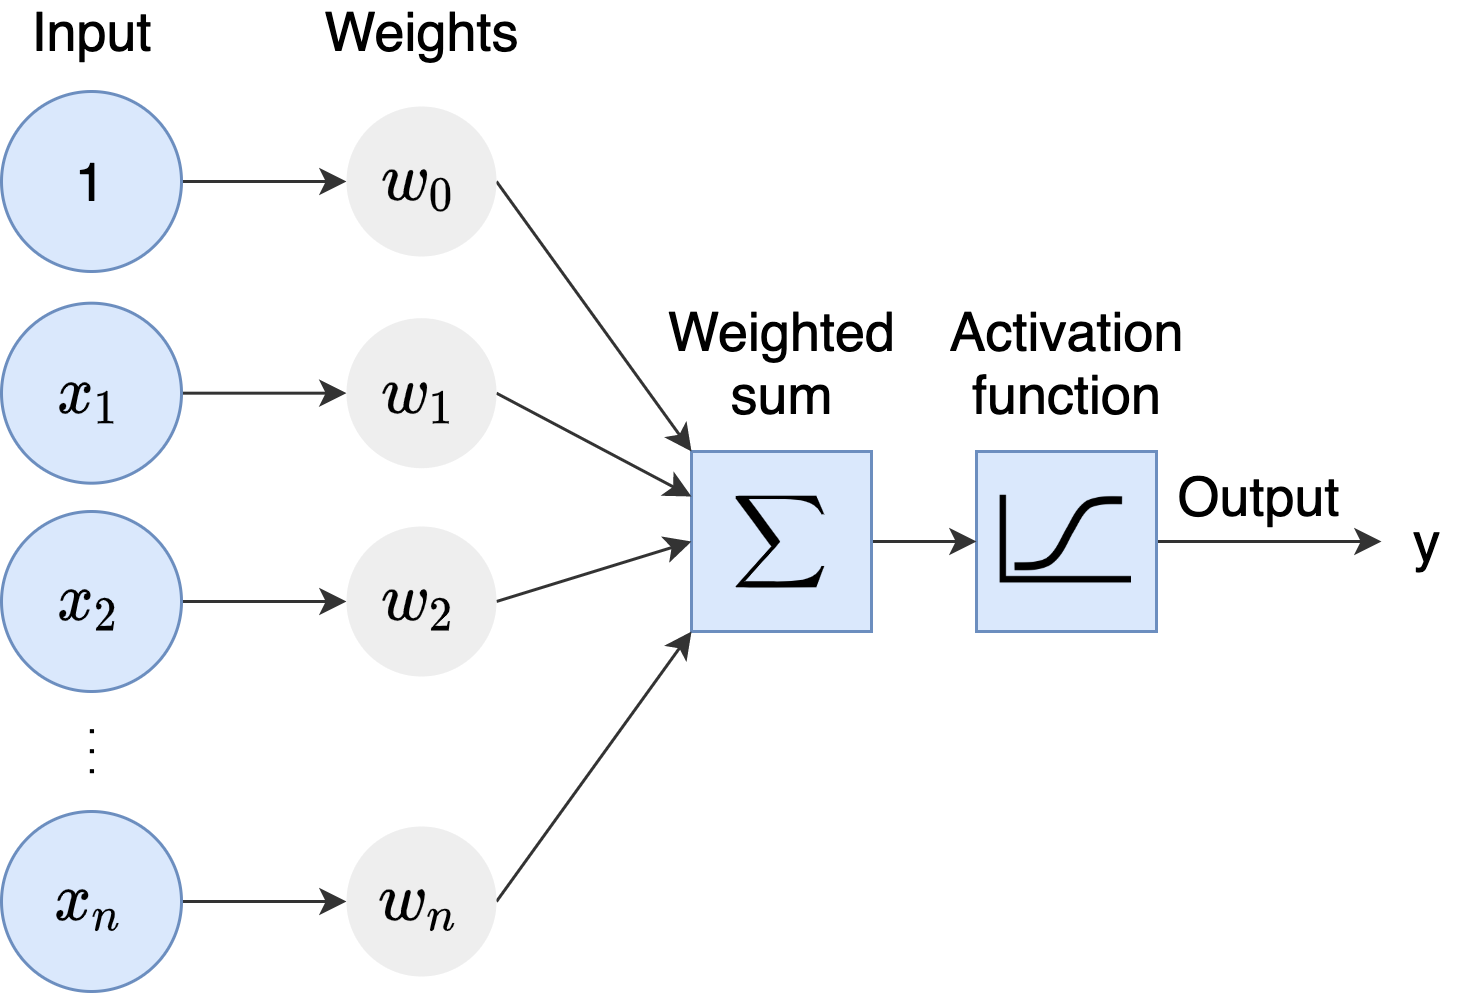
\includegraphics[width=0.7 \linewidth]{images/perceptron.png}
    \caption{A perceptron}
    \label{fig:perceptron}
\end{figure}

%All of the classifiers discussed below are categorised as \textit{Artificial Neural Networks} (ANNs), or just neural networks. An ANN, motivated by the human brain, is a collection of \textit{nodes}, or \textit{neurons}, which are connected through \textit{layers}. A layer consists of several nodes and, in its simplest form, a feed-forward layer, passes the information to (and only to) the next layer.

\paragraph{Perceptron} A \textit{perceptron} is a binary classifier and builds the basis for an \textit{Artificial Neural Network} (ANNs). An ANN, motivated by the human brain, is a collection of \textit{nodes}, or \textit{neurons}, which are connected through \textit{layers}. A layer consists of several nodes and, in its simplest form, a feed-forward layer, passes the information to (and only to) the next layer. 
Perceptron is the simplest form of ANN. It consists of only one neuron and outputs either $0$ or $1$. \cref{fig:perceptron} shows a perceptron that takes $n$-dimensional data as input. The output is computed by a linear combination of the input $\mathbf{X}=(x_1,x_2,\dots,x_n$) using the weights $\mathbf{w}=(w_0, \dots, w_n)$ 
\begin{align}
    \sum_{i=1}^n w_i x_i + w_0 = \mathbf{w}^\top \mathbf{X} + w_0
\end{align}
and applying a threshold step function with the threshold s
\begin{align}
    y = 
        \begin{cases}
        1 & \mathrm{for}\; \mathbf{w}^\top \mathbf{X} + w_0 \geq s\\
        0 & \mathrm{for}\;  \mathbf{w}^\top \mathbf{X} + w_0 < s
        \end{cases}.
\end{align}
During training, the weights of the perceptron are updated iteratively. Given a dataset consisting of example-label pairs $\mathcal{D} = \{(\mathbf{X}^1, y^1), (\mathbf{X}^2, y^2), \dots, (\mathbf{X}^k, y^k)\}$, we pass each example through the perceptron and update the weights according to the prediction. Let $\hat{y}^i$ be the predicted label for the input $\mathbf{X}^i$, then the weights are updated by
\begin{align*}
w_i^{\mathrm{new}} = w_i + \alpha (y^i - \hat{y}^i)x_i, \quad i=1, \dots n, 
\end{align*}
where $\alpha$ is the learning rate, which is an instance of the hyperparameters. This process is repeated until the prediction is correct for all examples in the dataset.
More complex types of ANNs are discussed in the following section.

% http://alexlenail.me/NN-SVG/LeNet.html
\subsubsection{Deep Learning} \label{sec:deep-learning}
\begin{figure} %[H]
    \centering
    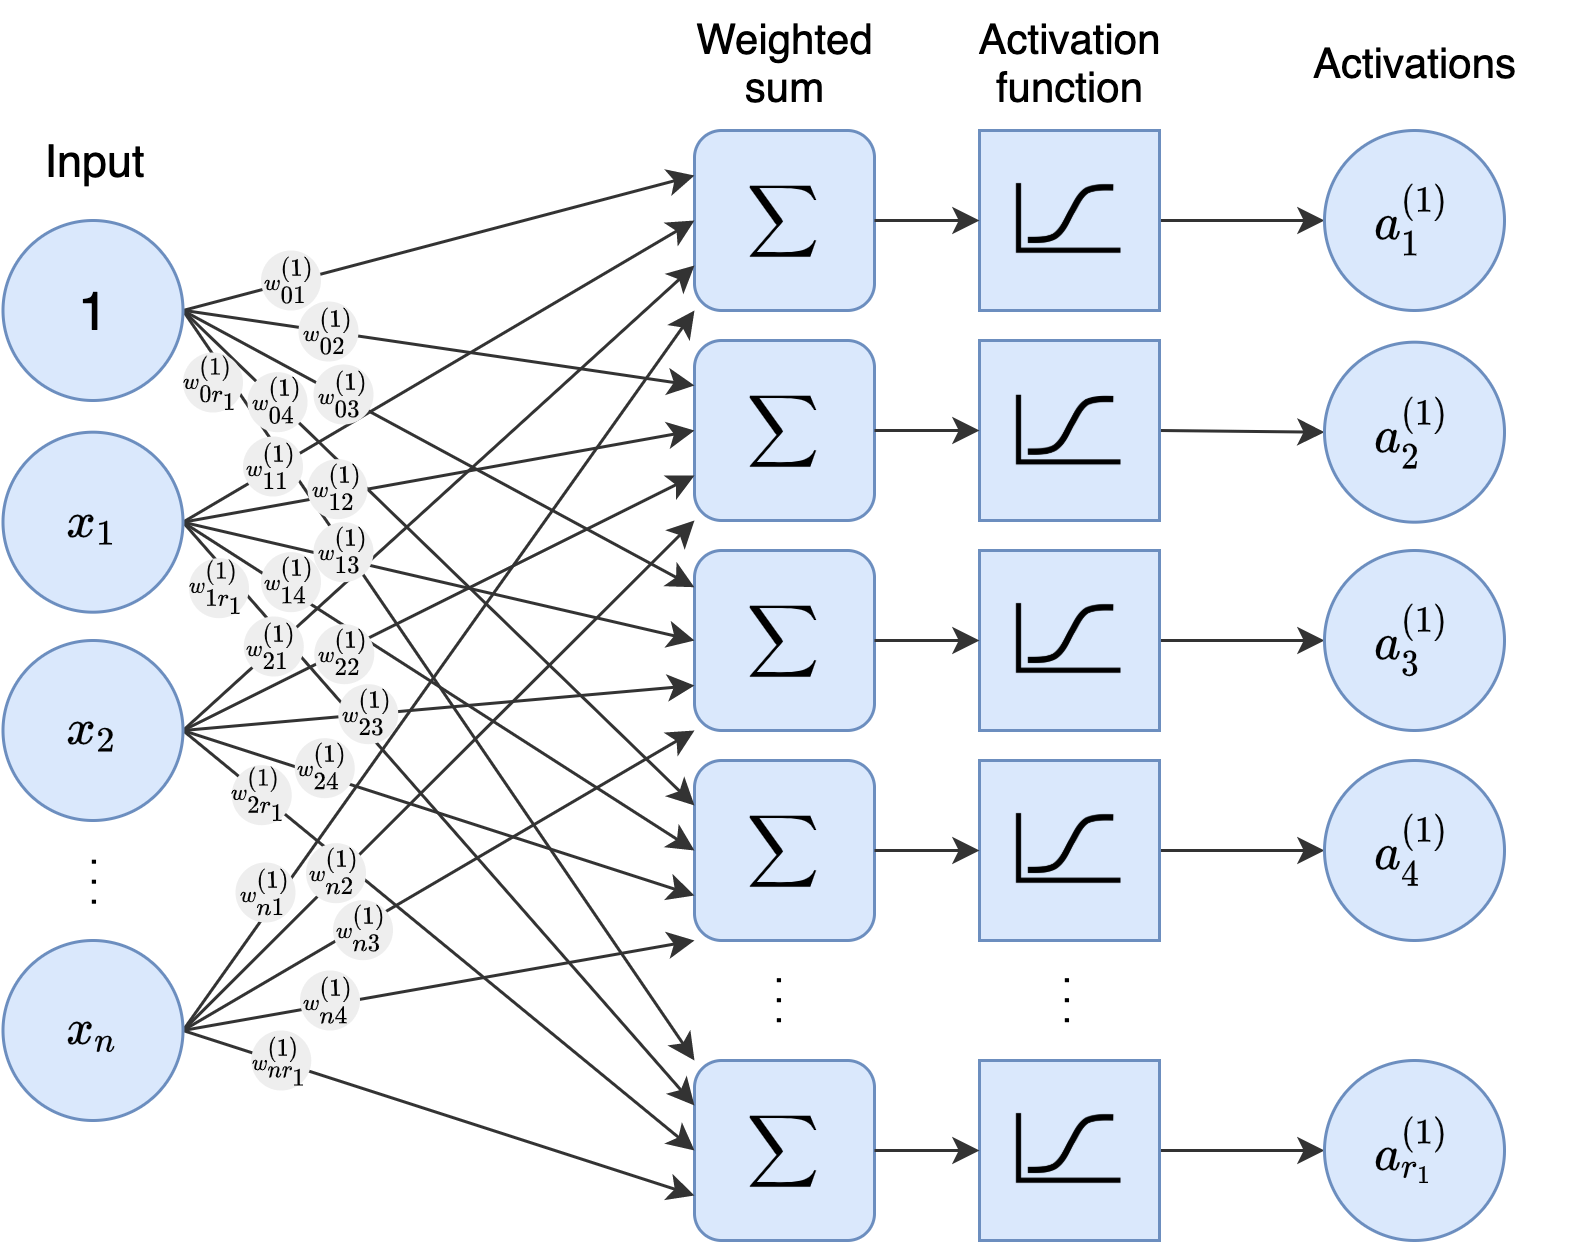
\includegraphics[width = 0.9\linewidth]{images/MLP.png}
    \caption{Computation of first layer in an MLP.}
    \label{fig:MLP}
\end{figure}

Deep Learning \cite{goodfellow_deep_2016} (DL) is a type of Machine Learning that achieves remarkable results on many tasks, by dividing a problem into many sub-problems. The basis for Deep Learning is a \textit{Multi-Layer Perceptron} (MLP). An MLP is a perceptron with at least one hidden layer. The hidden layer is again composed of perceptrons, as it is visualised in \cref{fig:MLP}. A feed-forward \textit{Deep Neural Network} (DNN) is an MLP with multiple (at least two) hidden layers. In general, the term DNN can be any ANN, not only MLP, with more than one hidden layer.
%The input layer is connected via hidden layers to the output layer which indicates the predicted label. \Cref{fig:neural_network} shows an illustration of a DNN.

We will now explain the computations in an MLP, but first we have to define the notation. We denote the model's parameters or weights with $\mathbf{w}$, but also $\theta$ is frequently used in other literature. As shown in \cref{fig:MLP}, we denote the input to a neural network as $\mathbf{X}= \left(x_1, x_2, \dots, x_n \right)^\top \in \mathbb{R}^n$, the weights connecting the input to the first node of the first hidden layer as $\mathbf{w}_1^{(1)} = \left(w_{11}^{(1)}, w_{21}^{(1)}, \dots, w_{n1}^{(1)} \right)^\top$, the weights connecting the input to the second node of the first hidden layer as $\mathbf{w}_2^{(1)} = \left(w_{12}^{(1)}, w_{22}^{(1)}, \dots, w_{n2}^{(1)} \right)^\top$, etc. Let $n$ be the size of the input and $r_1$ the size of the first hidden layer, then the weights for the first hidden layer can be combined into a matrix (and also analogously for all the other layers):
\begin{align}
\mathbf{W}^{(1)} = \left(\mathbf{w}_1^{(1)}, \dots ,\mathbf{w}_{r_1}^{(1)} \right) = \left(
\begin{array}{ccc} 
w_{11}^{(1)} & \cdots & w_{1r_1}^{(1)} \\ 
\vdots & \ddots & \vdots \\ 
w_{n1}^{(1)} & \cdots & w_{nr_1}^{(1)} \\ 
\end{array}
\right)
\end{align}

The first hidden layer's activations are denoted as $\mathbf{a}^{(1)} = \left(a_1^{(1)}, a_2^{(1)}, \dots, a_{r_1}^{(1)}\right)^\top$, the second hidden layer's nodes as $\mathbf{a}^{(2)} = \left(a_1^{(2)}, a_2^{(2)}, \dots, a_{r_2}^{(2)}\right)^\top$. The weights connecting $\mathbf{a}^{(1)}$ to $\mathbf{a}^{(2)}$ are denoted as $\mathbf{W}^{(2)}$. And finally, if the neural network consists of $L$ hidden layers, then the last hidden layer $\mathbf{a}^{(L)}$ is connected to the output layer $\mathbf{a}^{(O)}$ through $\mathbf{W}^{(L)}$. Let the size of the $l$-th layer be $r_l$.

With $g$ being the activation function, the first hidden layer's nodes are then computed as
\begin{align} 
    a_1^{(1)} &= g\left(\sum_{i=1}^{n} w_{i1}^{(1)} x_i + w_{01}^{(1)} \right) = g\left( {\mathbf{w}_1^{(1)}}^\top \mathbf{X} + w_{01}^{(1)} \right), \label{eq:first_layer_comp_1} \\
    &\vdots \nonumber \\
    a_{r_1}^{(1)} &= g\left(\sum_{i=1}^{n} w_{ir_1}^{(1)} x_i + w_{0r_1}^{(1)} \right) = g\left( {\mathbf{w}_{r_1}^{(1)}}^\top \mathbf{X} + w_{0r_1}^{(1)} \right), \label{eq:first_layer_comp_r1}
\end{align}
and directly fed into the computation for the second hidden layer:
\begin{align}
    a_1^{(2)} &= g\left(\sum_{j=1}^{r_1} w_{j1}^{(2)} a_j^{(1)} + w_{01}^{(2)} \right) = g\left(\sum_{j=1}^{r_1} w_{j1}^{(2)} g\left(\sum_{i=1}^{n} w_{ij}^{(1)} x_i + w_{0j}^{(1)} \right) + w_{01}^{(2)} \right), \label{eq:second_layer_comp_1} \\
    &\vdots \nonumber \\
    a_{r_2}^{(2)} &= g\left(\sum_{j=1}^{r_1} w_{jr_2}^{(2)} a_j^{(1)} + w_{0r_2}^{(2)} \right) = g\left(\sum_{j=1}^{r_1} w_{jr_2}^{(2)} g\left(\sum_{i=1}^{n} w_{ij}^{(1)} x_i + w_{0j}^{(1)} \right) + w_{0r_2}^{(2)} \right). \label{eq:second_layer_comp_r2}
\end{align}
Iteratively, we obtain the formula for the $l$-th node in the output layer:
\begin{align}
a_l^{(O)} &= g\left(\sum_{m=l}^{r_{L}} w_{ml}^{(O)} a_m^{(L)} + w_{0l}^{(O)} \right) \label{eq:last_layer_comp_1} \\
&= g\left(\sum_{m=l}^{r_L} w_{ml}^{(O)} \cdots g\left(\sum_{j=1}^{r_1} w_{jk}^{(2)} g\left(\sum_{i=1}^{n} w_{ij}^{(1)} x_i + w_{0j}^{(1)} \right) + w_{0k}^{(2)} \right) \cdots + w_{0l}^{(O)} \right) \label{eq:last_layer_comp_2}
\end{align}

The activation function $g$ decides, depending on the weighted sum, if a node should be activated or not, i.e. if the output of the node will be used for further computations or not. Common activation functions are the \textit{Heaviside step function}
\begin{align}
    g(x) = 
        \begin{cases}
        1 & \mathrm{for}\;  x \geq 0 \\
        0 & \mathrm{for}\; x < 0
        \end{cases},
\end{align}
a piecewise linear function, e.g., 
\begin{align}
    g(x) = 
        \begin{cases}
        1 & \mathrm{for}\; x \geq \frac{1}{2} \\
        x + \frac{1}{2} & \mathrm{for}\;  -\frac{1}{2} < x < \frac{1}{2} \\
        0 & \mathrm{for}\; x \leq -\frac{1}{2}
        \end{cases},
\end{align}
the \textit{sigmoid function} (which is used as a symbolic example in \cref{fig:MLP})
\begin{align}
    g(x) = \frac{1}{1+e^{-t}},
\end{align}
or, also a piecewise linear function, the \textit{Rectified Linear Unit} (ReLU) activation function
\begin{align}
    g(x) = \mathrm{max}(0,x).
\end{align}
The latter one is commonly used in Deep Learning, as only the neurons with a positive value are activated and therefore not all of them get activated at once as they would with a sigmoid function, being far more computationally efficient. There exist many other variations of ReLU, e.g. \textit{leaky ReLU} \cite{maas_rectifier_2013} and \textit{parameterised ReLU} (PReLU) \cite{he_delving_2015}, just to name a few. Leaky ReLU activates neurons also with a negative value, but weights it small:
\begin{align}
    g(x) = 
        \begin{cases}
        x & \mathrm{for}\;  x > 0 \\
        0.01x & \mathrm{for}\; x \leq 0
        \end{cases}
\end{align}
The PReLU takes the idea further and introduces a parameter which is learned during training:
\begin{align}
    g(x) = 
        \begin{cases}
        x & \mathrm{for}\;  x > 0 \\
        ax & \mathrm{for}\; x \leq 0,
        \end{cases}
\end{align}
with $a$ being the additional.

In order to solve the classification problem, we need a loss function that will be minimised during model training.
%Compared to the loss function in \cref{eq:regression_loss}, we cannot measure a "distance" between the predicted value and the true value by computing the mean squared error. Therefore, t
The function that is commonly used in classification is the \textit{Categorical Cross Entropy loss} function. It is used whenever an output vector is returned instead of one label. First, the \textit{Softmax} function $S$ is applied to the output vector to get output probabilities, i.e. values between 0 and 1, with the highest value corresponding to the model's prediction:
\begin{align}
    S\left(a^{(O)}_i\right) = \frac{\exp a^{(O)}_i}{\sum_j \exp a^{(O)}_j}
\end{align}
Given the input $\mathbf{X}$, a one-hot encoded label vector $\mathbf{y}=(y_1,y_2, \cdots, y_C) \in \{0,1\}^C$, where $C$ is the number of classes in the model, and the output vector of the model $\mathcal{F}_{\mathbf{W}}(\mathbf{X})=\mathbf{a}^{(O)}(\mathbf{X})$, the categorical cross entropy loss is then computed by
\begin{align}
    \mathcal{L}(\mathcal{F}_{\mathbf{W}}(\mathbf{X}), \mathbf{y}) &= - \sum_{i}^C y_i \log \left( \frac{\exp a^{(O)}_i(\mathbf{X})}{\sum_j \exp a^{(O)}_j(\mathbf{X})} \right) \\
    &= - \log \left( \frac{\exp a^{(O)}_p(\mathbf{X})}{\sum_j \exp a^{(O)}_j(\mathbf{X})} \right) \\
    &= - \log \left( S\left(a^{(O)}_p\right) \right),
\end{align}
with $p$ being the position in the output vector corresponding to the true label. The second equation holds since the label vector is one-hot encoded and all of the other terms are cancelled out. Therefore, the cross entropy loss returns high values for a small value in the output probabilities vector and vice versa, working as a penalty function. A perfect prediction with a one-hot encoded output probabilities vector would results in a loss of zero, which the model aims to learn during training. 

Since the output vector $\mathbf{a}^{(O)}$ mainly depends on the weights $\mathbf{W} = (\mathbf{W}^{(1)}, \mathbf{W}^{(2)}, \dots, \mathbf{W}^{(L)})$ of the DNN, we can formulate the optimisation problem for the DNN as
\begin{align}
    \min_{\mathbf{W} \in \mathbb{R}^{m}} \mathcal{L}(\mathbf{W},\mathcal{F}_{\mathbf{W}}(\mathbf{X}), \mathbf{y}) = \max_{\mathbf{W} \in \mathbb{R}^{m}} \log \left( \frac{\exp a^{(O)}_p}{\sum_j  \exp a^{(O)}_j} \right),
\end{align}
where here $\mathbf{W} \in \mathbb{R}^m$ denotes the flattened version of the matrix $\mathbf{W}$ with length $m = nr_1 + \sum_{i=2}^L r_{i-1}r_i$.

In order to solve this optimisation problem, a multitude of optimisation algorithms has been introduced \cite{goodfellow_deep_2016}. \textit{Gradient descent} is the most basic gradient-based optimisation algorithm and forms the basis for the more advanced ones. The algorithm updates the parameters after computing the gradients based on the whole training set and is therefore not recommended to use with large datasets. Let $\mathcal{D} = \{(\mathbf{X}^1, y^1), (\mathbf{X}^2, y^2), \dots, (\mathbf{X}^k, y^k)\}$ the training set, then the update rule for the parameters is as follows
\begin{align}
    \mathbf{W}^{\mathrm{new}} = \mathbf{W} + \alpha \nabla_{\mathbf{w}} \sum_{i=1}^k \mathcal{L}(\mathbf{W},\mathcal{F}_{\mathbf{W}}(\mathbf{X}^i), y^i),
\end{align}
where $\alpha$ denotes the learning rate. The algorithm converges even with a fixed learning rate, provided that the gradients of the loss function are Lipschitz continuous.

A more commonly used algorithm is the \textit{Stochastic Gradient Descent} (SGD), which estimates the gradients based on a batch of training samples. Given a batch of $m$ training samples $\{(\mathbf{X}^1, y^1), (\mathbf{X}^2, y^2), \dots, (\mathbf{X}^m, y^m)\}$, the gradient estimate is computed by
\begin{align}
    \hat{\mathbf{g}} = \frac{1}{m} \sum_{i=1}^m \mathcal{L}(\mathbf{W},\mathcal{F}_{\mathbf{W}}(\mathbf{X}^i), y^i)
\end{align}
and the parameters are updated after running through a batch by
\begin{align}
    \mathbf{W}^{\mathrm{new}} = \mathbf{W} - \alpha \hat{\mathbf{g}}.
\end{align}

Another widely used algorithm is the \textit{Adam} optimiser \cite{kingma_adam_2015}, which is an extension of the SGD. Adam is an adaptive gradient descent algorithm, i.e. it adapts the learning rate per parameter. Some models tend to perform better optimised with Adam than with SGD.

\textit{Learning rate schedulers} adapt the (global) learning rate during training, dependent on the number of iterations, according to a pre-defined schedule. Two commonly used learning rate schedulers are \texttt{MultiStepLR} and \texttt{CosineAnnealingLR}. \textit{MultiStepLR} reduces the learning rate every $n$ epochs by a rate of, e.g., 0.1. The learning rate gets smaller every $n$ epochs. \textit{CosineAnnealingLR}, however, has a schedule that decreases the learning rate but also increases, in an overall downward trend.

\textit{Convolutional Neural Networks} (CNNs) \cite{krizhevsky_imagenet_2017} are a special type of DNNs where the hidden layers consist of convolutional, pooling and feed-forward layers. CNNs achieved a breakthrough in image recognition. The convolutional filters are applied to the image and enhance special features in an image, e.g. edges, lines or different shapes, and make it therefore possible to learn how to distinguish between objects. A schematic view of this process is shown in \cref{fig:cnn_features}.

\begin{figure}
    \centering
    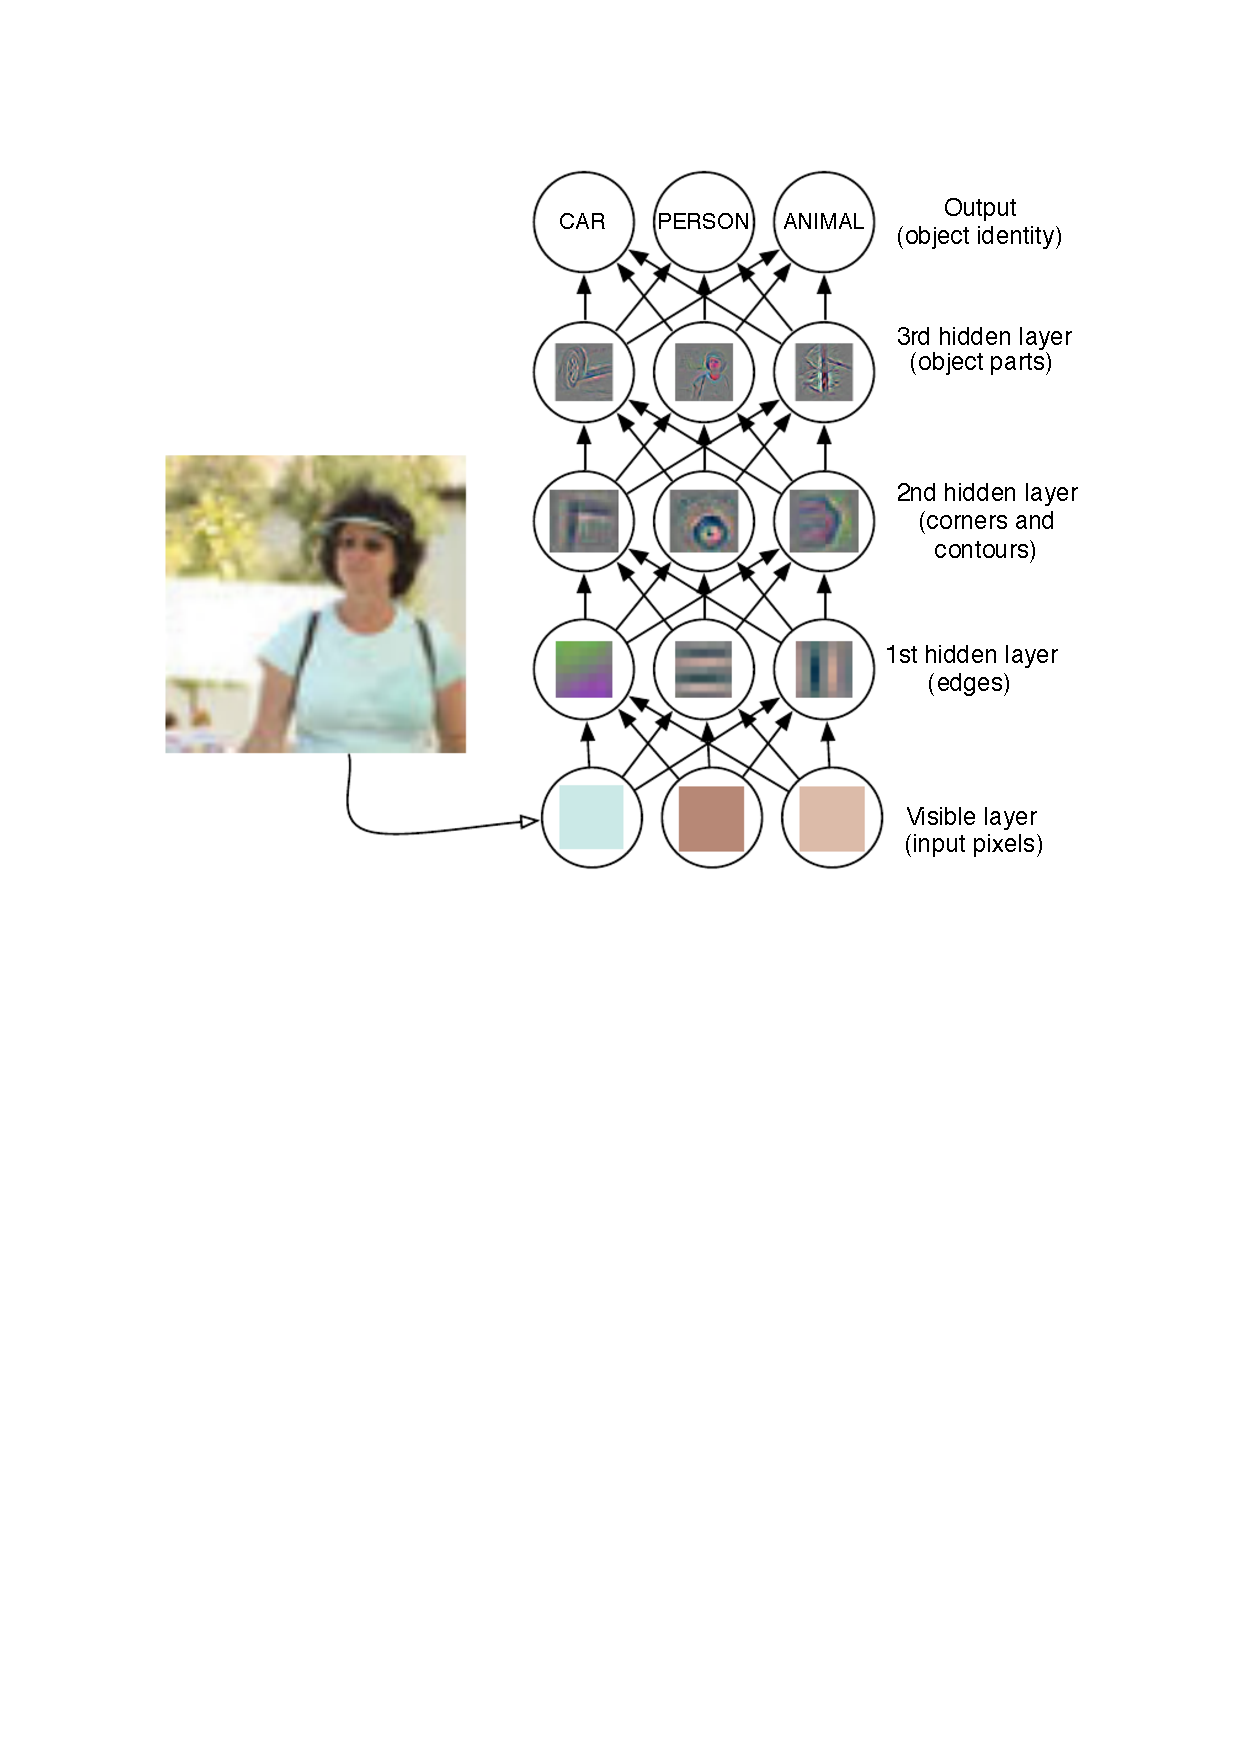
\includegraphics[width=0.7 \textwidth]{images/cnn_features.pdf}
    \caption{Convolutional filters in a Deep Neural Network enhancing features in an image. Usually, the first layers recognise simple features such as lines and corners by comparing the contrast of neighbouring pixels. With this information, the following layers are responsible for recognising whole object parts. In this manner, feeding the pixel information from the input through a series of layers consisting of convolutional, pooling and feed-forward layers, eventually results in a class prediction. Source: \cite{goodfellow_deep_2016}}
    \label{fig:cnn_features}
\end{figure}

Convolutional layers \cite{goodfellow_deep_2016} differ in computation compared to ordinary feed-forward layers as shown before in \cref{eq:first_layer_comp_1,,eq:first_layer_comp_r1,eq:second_layer_comp_1,eq:second_layer_comp_r2,eq:last_layer_comp_1,eq:last_layer_comp_2}. Convolutional layers consist of one of more convolutional \textit{filters} or \textit{kernels}. As the name already indicates, the layer performs a mathematical operation called convolution, which we would like to explain in detail. The following definitions are adapted from \cite{goodfellow_deep_2016}. The \textit{continuous mathematical convolution} is an operation on two functions of real arguments, say $f,g: \mathbb{R}^n \to \mathbb{C}$, and computed as
\begin{align}
    (f \ast g) (x) := \int_{\mathbb{R}^n} f(y) g(x-y)dy.
\end{align}
The mathematical convolution is a weighted mean value, for which every $f(y)$ is weighted by $g(x-y)$. If we deal with discrete functions, which for computational reasons is necessary, we define the \textit{discrete mathematical convolution} as
\begin{align}
    (f \ast g) [x] := \sum_{y=-\infty}^{\infty} f[y] g[x-y].
\end{align}
In Machine Learning, however, a \textit{convolution} performs a slightly different operation. Since we usually deal with multi-dimensional input data, e.g. images, of finite size, let the input $\mathbf{X} \in \mathbb{R}^{n \times n}$ and the kernel $\mathbf{K} \in \mathbb{R}^{m \times m}$ be two-dimensional and finite. Then, the convolution is computed as
\begin{align}
    (\mathbf{I} \ast \mathbf{K})[i,j] = \sum_m \sum_n \mathbf{I}[i+m,j+n] \mathbf{K}[m,n], \quad 1 \leq i,j \leq n-m+1
\end{align}
and the output is called \textit{feature map}. A schematic view of the computation is shown in \cref{fig:convolution}. Depending on the values of a kernel, the image is processed in a different way, in order to enhance the special features in an image. Those values of a kernel are iteratively updated during training, i.e. the model learns how to enhance features in order to distinguish between different objects. In this way, a CNN is able to classify images depending on special features in an image and therefore better at generalisation compared to image classification with an MLP.

%\red{TODO: show convolution filters for enhancement of horizontal/vertical lines}

Pooling layers \cite{goodfellow_deep_2016} serve as a summary of information after a convolutional layer. They reduce the dimension of data and help to make the representation become invariant to small changes in the input. Common pooling techniques are \textit{max} and \textit{average} pooling. Max pooling takes the maximum value within a rectangular neighbourhood and average pooling takes the average value.

%\red{TODO: Show 1-2 examples of current CNN architectures (do you show that later?)}


\begin{figure}
    \centering
    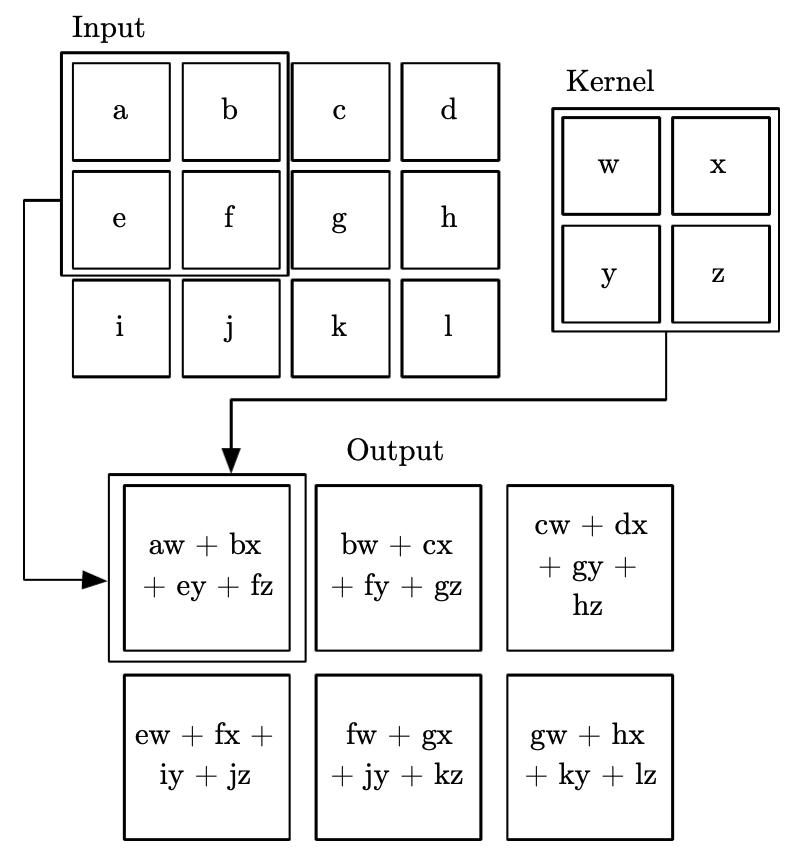
\includegraphics[width= 0.5 \textwidth]{images/convolution_deeplearning.png}
    \caption{Computation of convolutional filter with padding 1. Padding means how much the filter shifts on the input during the computation. With padding 2, e.g., the filter would move forward two values instead of one, in order to compute the next output value. Source: \cite{goodfellow_deep_2016}}
    \label{fig:convolution}
\end{figure}

\textit{Recurrent Neural Networks} \cite{rumelhart_learning_1986} (RNNs) are another special type of DNNs where the connections between neurons are not only limited to the neighbouring layer, like in feed-forward neural networks but can be connected to any other neuron and therefore forming a "memory" for the network. RNNs support sequential data and are especially important for non-static problems like speech recognition. Famous RNNs are the Long Short-Term Memory Network (LSTM) \cite{hochreiter_longshorttermmemory_1997} and Gated Recurrent Unit (GRU) \cite{cho_learning_2014}. \cref{fig:lstm_gru} shows an illustration for LSTM and GRU. LTSMs and GRUs have internal mechanisms called \textit{gates} that can regulate the flow of information. The gates are trained to distinguish which data in a sequence is important and which is not.

%source: https://towardsdatascience.com/illustrated-guide-to-lstms-and-gru-s-a-step-by-step-explanation-44e9eb85bf21
\begin{figure}
    \centering
    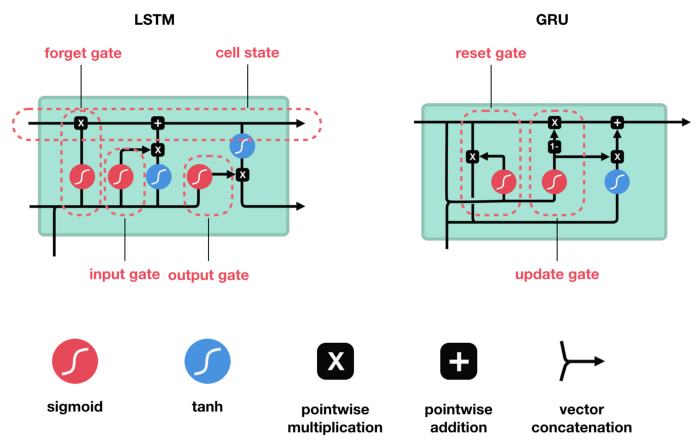
\includegraphics[width= 0.8 \linewidth]{images/LSTM_and_GRU.png}
    \caption{LSTM and GRU. Source: \cite{phi_illustrated_2018}}
    \label{fig:lstm_gru}
\end{figure}


%Common algorithms in Supervised Learning are \textit{Support Vector Machine} (SVM), \textit{Random Forest} and \textit{(Artificial) Neural Networks} (ANNs), especially \textit{Deep Neural Networks} (DNNs). A DNN is an feed-forward ANN with multiple fully-connected hidden layers. 


%https://towardsdatascience.com/https-medium-com-piotr-skalski92-deep-dive-into-deep-networks-math-17660bc376ba


%TODO: present examples of CNNs: LeNet \cite{lecun_gradient-based_1998}, AlexNet \cite{krizhevsky_imagenet_2017}, VGG \cite{simonyan_very_2014}, ResNet \cite{he_deep_2016} and DenseNet \cite{huang_densely_2017}, GoogLeNet
%TODO: examples RNN: Long Short-Term Memory Network (LSTM) \cite{hochreiter_long_1997} and Gated Recurrent Unit (GRU) \cite{cho_learning_2014}

%TODO: describe Graph Neural Networks, because it will be mentioned later. Daryna wrote: A \textit{Graph Neural Network} (GNN) is used to process the data represented in a graph structure \cite{scarselli_graph_2009}. The most famous application of such type of networks is Social Network Analysis (SNA). GNNs allows performing node classification, link prediction, or complete graph classification.


\subsubsection{Fine-Tuning}
% Fine-tuning with new data: Ross Girshick, Jeff Donahue, Trevor Darrell, and Jitendra Malik. 2014. Rich feature hierarchies for accurate object detection and semantic segmentation. In Proceedings of the IEEE conference on computer vision and pattern recognition. 580–587.
The process of \textit{Fine-Tuning} \cite{girshick_rich_2014}, training a model on different training data with a smaller learning rate, can be used for either improving the model or when using it for a slightly different purpose, in \textit{Transfer Learning} \cite{pan_survey_2010}. In this thesis, we use it either to embed a watermark or as a malicious modification to a well-trained model to remove unwanted information, e.g. a watermark.

\subsubsection{Overfitting} \label{sec:overfitting}
In training an ML model, \textit{overfitting} \cite{ying_overview_2019} is a common phenomenon. Overfitting means that the model is well-trained on the training data, but performs poorly on data that it has not seen before, e.g. the test set. Usually, this happens when the architecture is complex, but there is too little training data available. In this sense, the model has enough degrees of freedom so that it can "memorise" the training data rather than learn how to generalise.

One technique to prevent overfitting in ML models is \textit{regularisation} \cite{ying_overview_2019}. During model training, a \textit{parameter regulariser} is used. A regulariser is an additional term in a loss function, often in the form of a penalty term that controls the magnitude of the parameter values. The loss function $\mathcal{L}(\mathbf{w})$ with a regulariser is defined as
\begin{equation}
    \mathcal{L}(\mathbf{w}) = \mathcal{L}_0(\mathbf{w}) + \lambda \mathcal{L}_R(\mathbf{w}),
\end{equation}
where $\mathbf{w}$ is the parameter vector, $\mathcal{L}_0$ is the original loss function, $\mathcal{L}_R$ the regularisation term, and $\lambda$ an adjustable parameter. Several regularisers have been studied in the literature, e.g. the  $L_2$-regularisation, also called Ridge regularisation, or the $L_1$-regularisation, also called LASSO regularisation.

Another technique to prevent overfitting is \textit{early-stopping} \cite{ying_overview_2019}. During model training, the time when the model starts to overfit can be detected. It happens when the test or validation accuracy stops improving, but the train accuracy still does. With early-stopping, we stop the training when the validation loss is minimal. Since we only know that the validation loss is at its minimum when we train several iterations after we reached the minimum. An additional parameter for early-stopping is the \textit{patience}, the number of training iterations after the minimal validation loss was found, to confirm that this is indeed the right timing to stop training.

\subsubsection{Parameter Pruning}
Parameter pruning \cite{han_learning_2015} is a model compression technique, i.e. it is used to compress the model in order to reduce the storage and computation of the model. It has been shown that by applying parameter pruning, the number of parameters drops by a magnitude without any significant accuracy loss. The model parameters with the smallest absolute value are set to zero because one assumes that the weights with minimal values hold no or negligible information and can be cut out. In this thesis, we consider parameter pruning as either a targeted attack, as the attacker could assume that the pruned weights hold watermark information or as an accidental attack when the attacker wants to drop redundant parameters for storage reasons.

\subsection{Further ML techniques}
In the following, we introduce ML techniques that are mentioned in the thesis, but not as much of importance to the core work.

\textit{Federated Learning} \cite{yang_federated_2019} is an ML technique where multiple parties are involved in training the model on their data, without exchanging the data among each other, mostly for privacy-preserving goals.

\textit{Generative Adversarial Networks} (GANs) \cite{goodfellow_generative_2014} are an ML architecture that uses two DNNs to learn a task -- one DNN actually learns the task (the generator) and the other evaluates it (the discriminator). For instance, a common application area is picture generation. The generator learns to create pictures from scratch of, e.g. humans, and the discriminator evaluates its performance by comparing a set of real samples with the generated set. The discriminator has two possible outputs "real" and "fake". The goal of a GAN is that the discriminator outputs "real" for the images generated with the generator.

% todo: include img for GAN?

% autoencoder kommt vor in \cite{namba_robust_2019}
An \textit{autoencoder} is a special ANN that is commonly used for dimensionality reduction, that is to find a low-dimensional representation of high-dimensional data in an unsupervised manner. This is achieved by learning to copy its input to its output. It consists of an encoder and a decoder, and an internal (hidden) layer that describes a code learned to represent the input.

Knowledge \textit{Distillation} \cite{hinton_distilling_2015} is a type of compression technique that uses knowledge of a neural network (teacher network) to train a new smaller network (student network). A smaller model is computational less expensive and thus more appealing.

%Daryna wrote: Knowledge distillation~\cite{bucilua_model_2006,hinton_distilling_2015} is a model compression~\cite{cheng_survey_2017} method that allows to train a smaller network, using an already trained bigger network without decreasing accuracy. Usually, the bigger and smaller network are called teacher and student network, respectively. The main idea of this approach is that the student network is learning to duplicate the outputs of the teacher network on \textit{each} layer, not only the final output. This approach assumes white-box access to the teacher network, i.e. the architecture and model's weights \unsure{parameters is likely the better term} should be known.

\textit{Adversarial Examples} \cite{szegedy_intriguing_2014} are a kind of input that is created to fool a model. Usually, an original input (e.g. an image) is perturbed by some specially crafted noise such that the model is unable to classify the generated input correctly. The perturbation is kept minimal, to ideally not be noticeable by a human, or detection methods. Several methods to create Adversarial Examples have been proposed, the most well-known likely being the Fast Gradient Sign Method (FGSM) \cite{goodfellow_explaining_2015}.

\subsection{Model Extraction Attack}

A specific attack against the IP of ML models is the so-called \textit{Model Extraction Attack} (or Model Stealing Attack) \cite{tramer_stealing_2016}, which aims to reveal a model's internal characteristic or copy a complete model by only querying its API service. The target can be the architecture, parameters, decision boundary, functionality, or training hyper-parameters of the model.
% \cite{szyller_dawn_2020} has a nice section for model extraction.

\section{Watermarking} \label{sec:background:watermarking}
Digital watermarking is a well-studied procedure in e.g. multimedia Intellectual Property Protection (IPP) \cite{kahng_watermarking_1998} or relational databases \cite{kamran_comprehensive_2018}. The main idea is to embed a piece of signature in the data, e.g. image or audio, to deter malicious usage. This signature is often intended to be unnoticeable, however, perceptible watermarks are also commonly used in the multimedia domain; examples are logos or copyright notices that are added to images or videos to identify the author.
Non-perceptible watermarks, on the other hand, aim to avoid changing the perceptible impression of the data. This is also the type of watermark that we consider for the IPP of ML models. Digital watermarking is thus a form of steganography or information hiding, i.e. the practice of concealing a message within another message.
The hidden information must be embedded in such a way that no algorithm can remove or overwrite the watermark. Some recent digital watermarking techniques, e.g. for images, make use of DNNs in the embedding process \cite{zhong_automated_2020}; similarly, also attacks targeted to remove such watermarks are increasingly using deep learning techniques \cite{sharma_robust_2020}.

%Quiring et al. \cite{quiring_adversarial_2018}, for example, combines methods from model stealing to generate a \textit{substitute} model of a watermark detector, and then generates adversarial examples against this model, to obtain images with minimal perturbations that evade detection.

%Something like this should be somewere... but skipped for now
%Watermarking schemes for relational databases can as simplistic approach also be employed for white-box watermarking of ML models, as the parameters of these models can in most cases be represented as relational data.

In this thesis, we discuss (ML) model watermarking, i.e. the IP that has to be protected is an ML model. Model watermarking is related to multimedia or relational data watermarking, but the techniques differ since the protecting instance changed. 
Research on watermarking DNNs predominantly addresses image classification (cf. \cref{ch:sota}). The introduced terminology is thus strongly influenced by this application of ML, but we believe that the concepts are transferable to other input types as well.

At this point, we want to define the terminology that is common in model watermarking and is used throughout this work. A typical watermarking workflow is shown in \cref{fig:watermarking_workflow}. Watermark \textit{embedding} describes the process in which the watermark is placed into the model, e.g. via fine-tuning. We call watermark \textit{extraction} the process in which the embedded watermark is extracted from the model, but neither in a permanent (which is called \textit{watermark removal}) nor in a malicious way (which is called \textit{watermark detection}). Watermark extraction means that we want to identify if any, and which watermark is placed. 

Finally, during watermark \textit{verification}, the extracted watermark is compared to the model owner's watermark in order to prove ownership. Following certain rules (e.g. thresholding the watermark accuracy or (bit) error rate), it is then decided if the watermarks are the same.

\begin{figure}
    \centering
    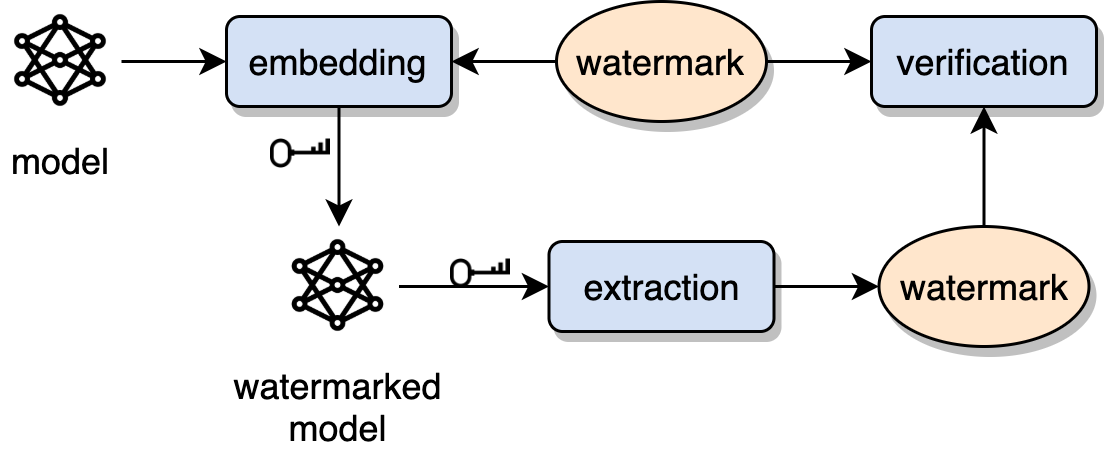
\includegraphics[width= 0.7\linewidth]{images/watermarking_workflow.png}
    \caption{A typical watermarking workflow}
    \label{fig:watermarking_workflow}
\end{figure}

\section{Fingerprinting}
We can consider fingerprinting as an extension of watermarking. While watermarking has the purpose to verify the \textit{owner} of a digital resource, fingerprinting wants to further trace back to the \textit{(malicious) recipient} of the resource. Therefore, fingerprinting techniques should be capable of embedding multiple, but unique, fingerprints in order to identify the recipient. These multiple fingerprints may be embedded in the same model, or in different versions of the model before distributing it.
%
Similar to watermarking, fingerprinting is already widely used in multimedia areas like images, audio and video \cite{lach_fpga_1998}, % Researchers extended the idea also to 
relational databases \cite{yingjiu_li_fingerprinting_2005}, and other digital data types.



%TODO: as discussed, move to a later section; also, distinguish between the concrete attacks that you have here, vs. what you call attacks in chapter 5 (SotA); in chapter 5, you rather have the *goal/aim* of the attack (or maybe the class), and here you have a specific attack (instance) (that might also achieve multiple goals at the same time..)
%----> done

%\section{Attacks}
%One of the most important requirements for a watermarking method is robustness (cf. \cref{sec:requirements}). In order to test robustness of the considered watermarking methods, we will perform two attacks, namely \textit{Fine-Tuning} and \textit{Parameter Pruning}. We have chosen those attacks, because a) these are the most common attacks performed in related work, and b) these are common steps to take when using a pre-trained model, e.g. in a transfer learning setting. A model user, regardless of whether malicious or not, could use fine-tuning for transferring the model to their task, and parameter pruning to compress the model.

%\subsubsection{Fine-Tuning}
% https://ruder.io/transfer-learning/
% https://machinelearningmastery.com/transfer-learning-for-deep-learning/
% https://medium.com/@14prakash/transfer-learning-using-keras-d804b2e04ef8
% https://builtin.com/data-science/transfer-learning

% Karen Simonyan and Andrew Zisserman. 2015. Very deep convolutional net- works for large-scale image recognition. In Proc. of ICLR.

%Transfer learning: Maxime Oquab, Leon Bottou, Ivan Laptev, and Josef Sivic. 2014. Learning and transferring mid-level image representations using convolutional neural net- works. In Proceedings of the IEEE conference on computer vision and pattern recognition.
%Some watermarking methods use fine-tuning \cite{girshick_rich_2014} to embed a watermark in a pre-trained model. Fine-tuning can be also seen as potential threat for the embedded watermark. Fine-Tuning can be either a targeted attack or an accidental attack: the attacker could perform fine-tuning for the purpose of Transfer Learning, or for purposely trying to remove the watermark by training on non-watermarked data. We will test the watermarking methods on the robustness against fine-tuning attacks 

%a model means that an already trained model is trained further on additional data with a smaller learning rate, usually for the purpose of Transfer Learning. In watermarking, some watermarking methods use fine-tuning to embed a watermark in a pre-trained model. We will mainly use fine-tuning as an attack and test the robustness of the watermarking methods, as we expect the (malicious) user to perform fine-tuning either for transfer learning or for purposely trying to remove the watermark. \red{CITE}

%\subsubsection{Parameter pruning}
% Song Han, Jeff Pool, John Tran, and William Dally. 2015. Learning both weights and connections for efficient neural network. In Advances in Neural Information Processing Systems. 1135–1143.


